\chapter{Pruebas y Resultados}

\section{Plan de Pruebas}

Las pruebas del sistema se realizaron sobre los flujos principales de iComanda,
validando los roles \texttt{admin}, \texttt{mesero}, \texttt{chef} y las rutas
públicas del cliente. La verificación fue funcional y exploratoria, revisando que
cada módulo cargue correctamente, permita completar sus acciones principales y se
integre con Supabase para lectura/escritura de datos.

\begin{center}
\renewcommand{\arraystretch}{1.25}
\small
\begin{tabular}{|p{1.4cm}|p{2cm}|p{4.2cm}|p{4.6cm}|p{1.8cm}|}
\hline
\textbf{ID} & \textbf{Rol} & \textbf{Caso} & \textbf{Resultado esperado} & \textbf{Estado} \\
\hline
CP-01 & General & Inicio de sesión & El usuario ingresa y es redirigido según su rol. & Superado \\
\hline
CP-02 & Admin & Gestión operativa & Se accede a usuarios, mesas, menú, pagos, gastos, reportes e inventario. & Superado \\
\hline
CP-03 & Mesero & Operación de pedidos & Se visualizan mesas, se crea pedido y se revisa detalle de orden. & Superado \\
\hline
CP-04 & Chef & Cocina & Se visualizan pedidos y se controla disponibilidad de platos. & Superado \\
\hline
CP-05 & Cliente & Carta y mesa pública & El cliente accede por URL/QR, ve el menú y puede llamar al mesero. & Superado \\
\hline
CP-06 & Gestión & Repositorio & Se evidencia control de versiones mediante GitHub y QR del repositorio. & Superado \\
\hline
\end{tabular}
\end{center}

\section{Evidencia de Interfaces y Resultados}

\subsection{Acceso al Sistema}

La pantalla de inicio de sesión valida el acceso de usuarios internos. Desde este
punto, el sistema redirige al módulo correspondiente según el rol cargado desde el
perfil del usuario.

\begin{figure}[H]
  \centering
  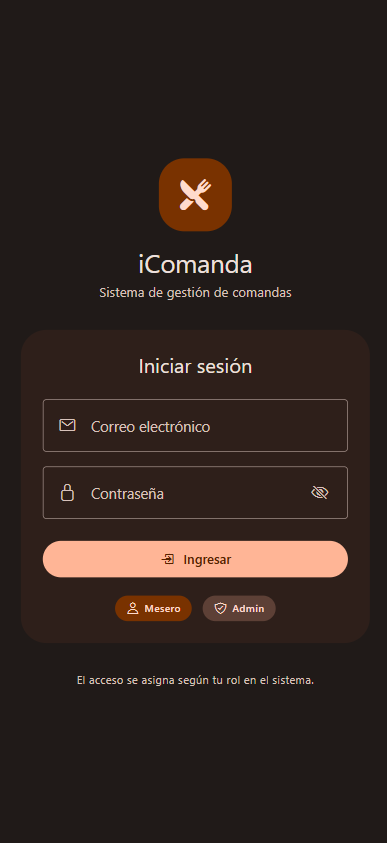
\includegraphics[width=0.35\textwidth]{img/login.png}
  \caption{Pantalla de inicio de sesión del sistema iComanda.}
\end{figure}

\subsection{Flujo de Administrador}

El administrador concentra la configuración operativa del restaurante. Las capturas
muestran el panel principal y la gestión del menú, diferenciando el acceso general
a módulos de la administración específica de platos.

\begin{figure}[H]
  \centering
  \begin{minipage}{0.48\textwidth}
    \centering
    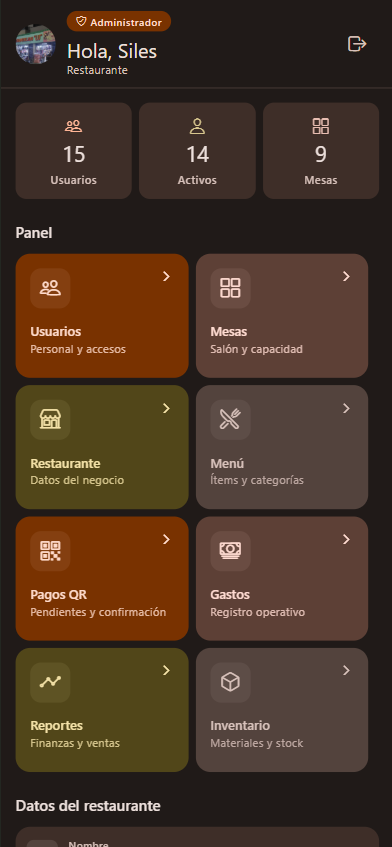
\includegraphics[width=0.92\linewidth]{img/admin-home.png}
  \end{minipage}
  \hfill
  \begin{minipage}{0.48\textwidth}
    \centering
    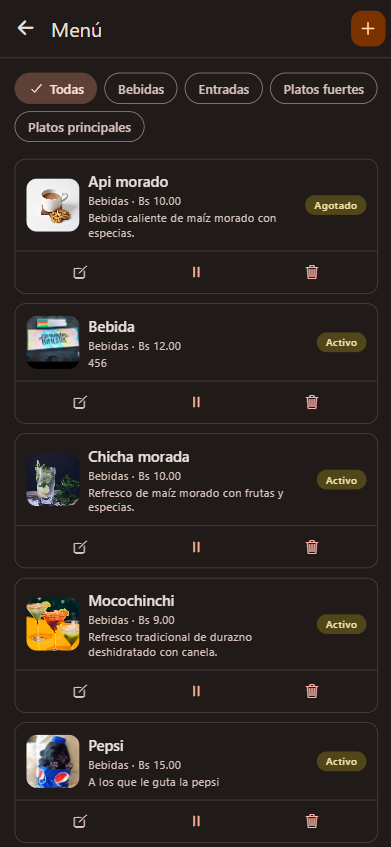
\includegraphics[width=0.92\linewidth]{img/admin-menu.png}
  \end{minipage}
  \caption{Panel principal del administrador y módulo de gestión de menú.}
\end{figure}

La administración también contempla usuarios, mesas y pagos QR. Estos módulos
permiten controlar el personal, la estructura física del restaurante y la validación
manual de pagos realizados mediante QR.

\begin{figure}[H]
  \centering
  \begin{minipage}{0.32\textwidth}
    \centering
    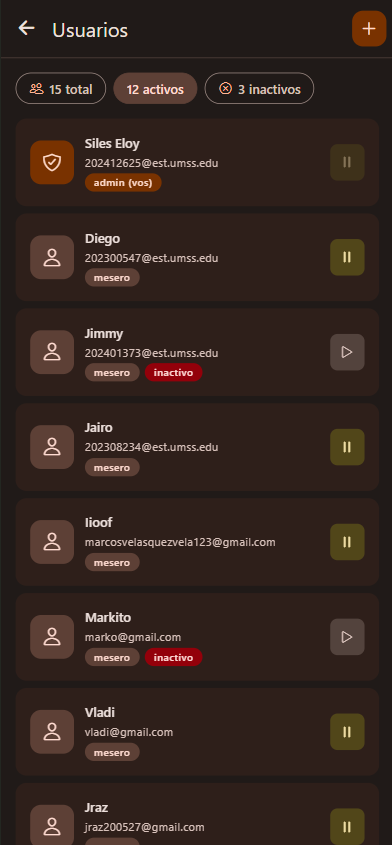
\includegraphics[width=0.95\linewidth]{img/admin-usuarios.png}
  \end{minipage}
  \hfill
  \begin{minipage}{0.32\textwidth}
    \centering
    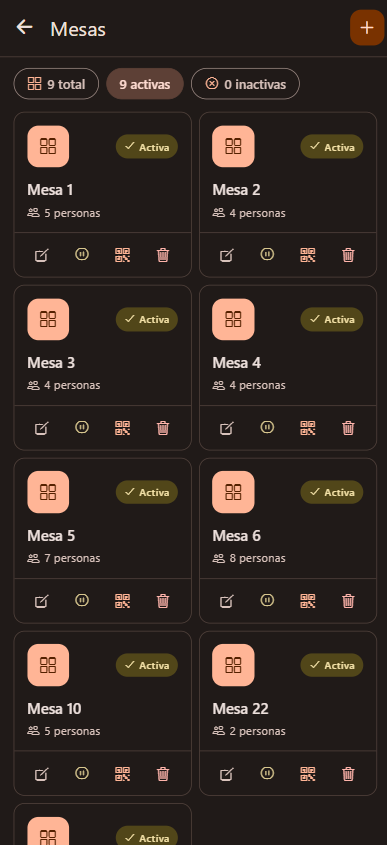
\includegraphics[width=0.95\linewidth]{img/admin-mesas.png}
  \end{minipage}
  \hfill
  \begin{minipage}{0.32\textwidth}
    \centering
    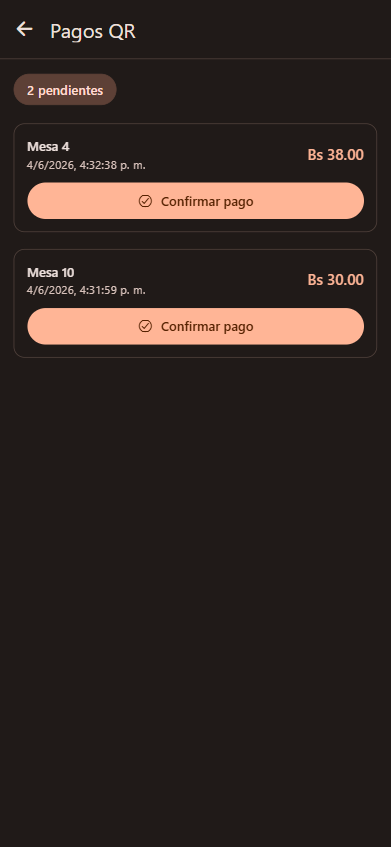
\includegraphics[width=0.95\linewidth]{img/admin-pagos.png}
  \end{minipage}
  \caption{Gestión administrativa de usuarios, mesas y pagos QR.}
\end{figure}

Los módulos financieros y de inventario permiten registrar egresos, analizar ventas,
consultar platos más vendidos y controlar materiales del restaurante.

\begin{figure}[H]
  \centering
  \begin{minipage}{0.48\textwidth}
    \centering
    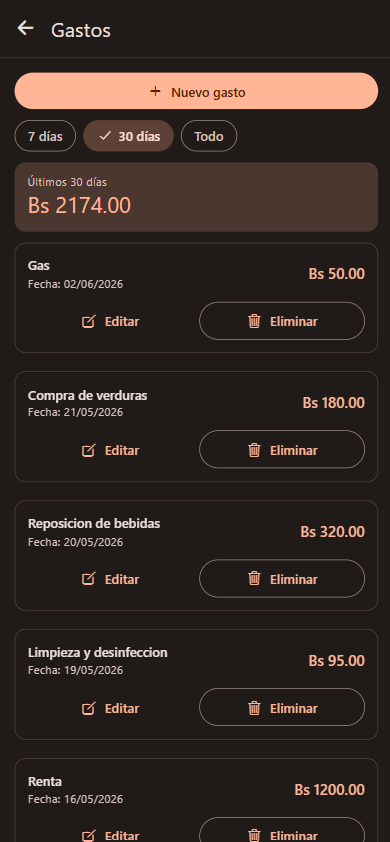
\includegraphics[width=0.92\linewidth]{img/admin-gastos.png}
  \end{minipage}
  \hfill
  \begin{minipage}{0.48\textwidth}
    \centering
    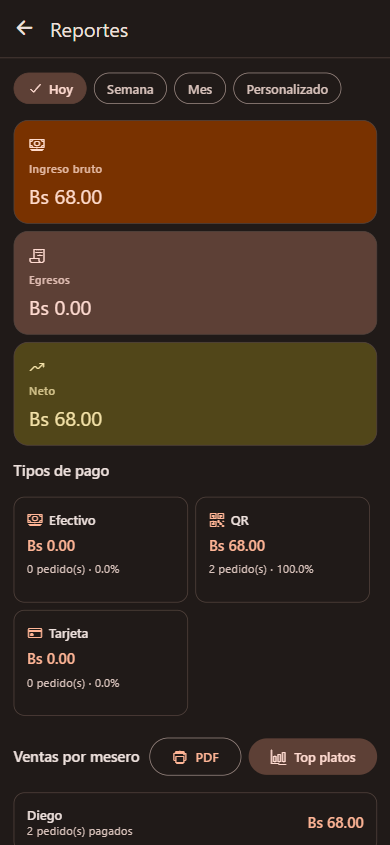
\includegraphics[width=0.92\linewidth]{img/admin-reportes.png}
  \end{minipage}
  \caption{Registro de gastos y visualización de reportes financieros.}
\end{figure}

\begin{figure}[H]
  \centering
  \begin{minipage}{0.48\textwidth}
    \centering
    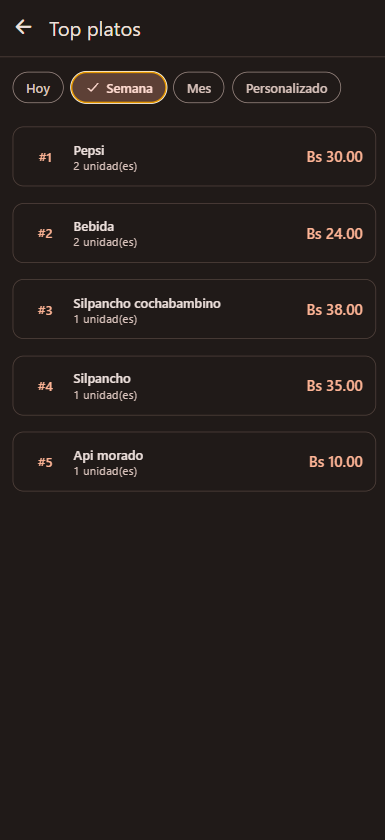
\includegraphics[width=0.92\linewidth]{img/admin-top.png}
  \end{minipage}
  \hfill
  \begin{minipage}{0.48\textwidth}
    \centering
    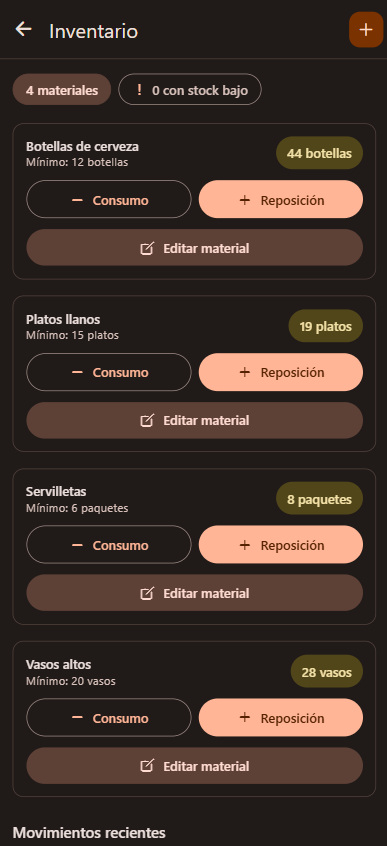
\includegraphics[width=0.92\linewidth]{img/admin-inventario.png}
  \end{minipage}
  \caption{Ranking de platos más vendidos e inventario de materiales.}
\end{figure}

\subsection{Flujo de Mesero}

El flujo de mesero valida la operación diaria: ver el estado de mesas, crear pedidos
y consultar el detalle de una orden. La vista de mesas se actualiza con los estados
operativos como libre, pendiente, listo, pendiente de pago, listo para limpiar o
cliente llama.

\begin{figure}[H]
  \centering
  \begin{minipage}{0.32\textwidth}
    \centering
    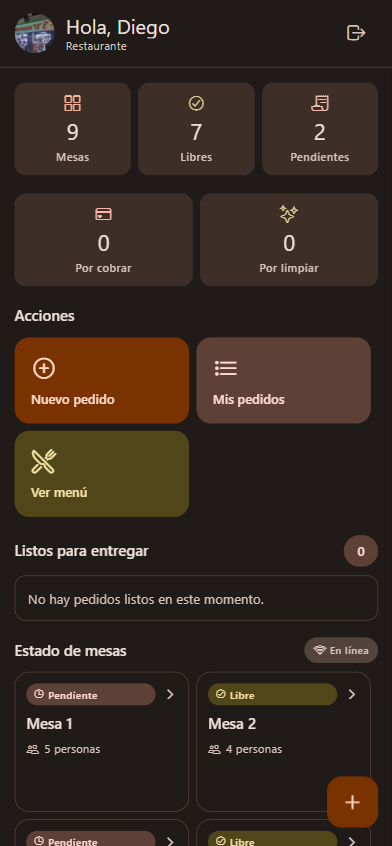
\includegraphics[width=0.95\linewidth]{img/mesero-home.png}
  \end{minipage}
  \hfill
  \begin{minipage}{0.32\textwidth}
    \centering
    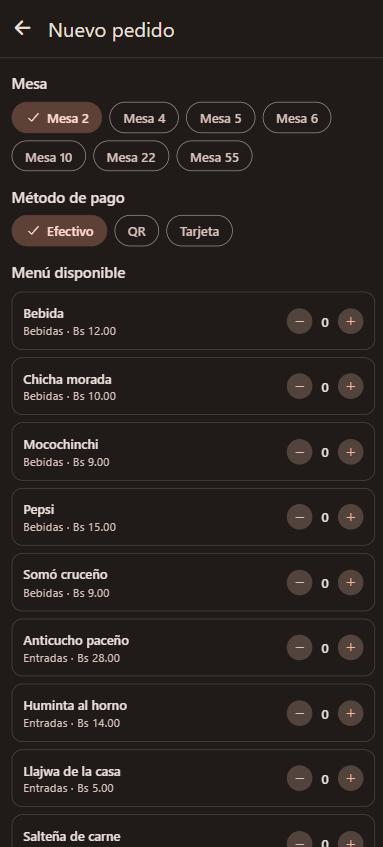
\includegraphics[width=0.95\linewidth]{img/mesero-pedido.png}
  \end{minipage}
  \hfill
  \begin{minipage}{0.32\textwidth}
    \centering
    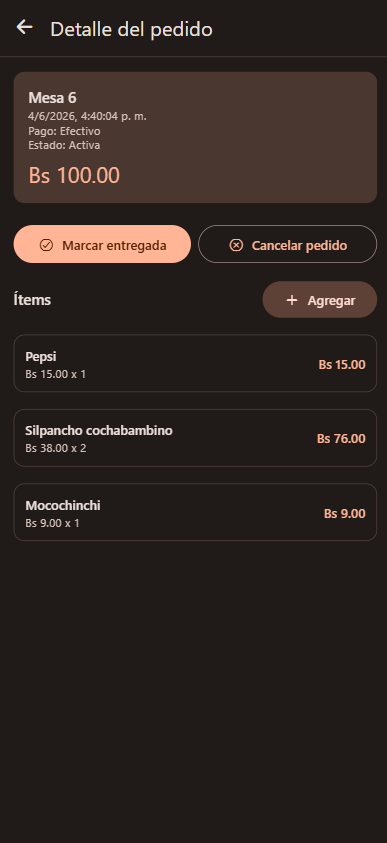
\includegraphics[width=0.95\linewidth]{img/mesero-detalle.png}
  \end{minipage}
  \caption{Vista de mesas, creación de pedido y detalle de orden del rol mesero.}
\end{figure}

\subsection{Flujo de Cocina}

El rol \texttt{chef} permite separar la operación de cocina del trabajo del mesero.
Desde esta interfaz se revisan pedidos en preparación, se marcan como listos y se
controla si un plato está agotado o disponible.

\begin{figure}[H]
  \centering
  \begin{minipage}{0.48\textwidth}
    \centering
    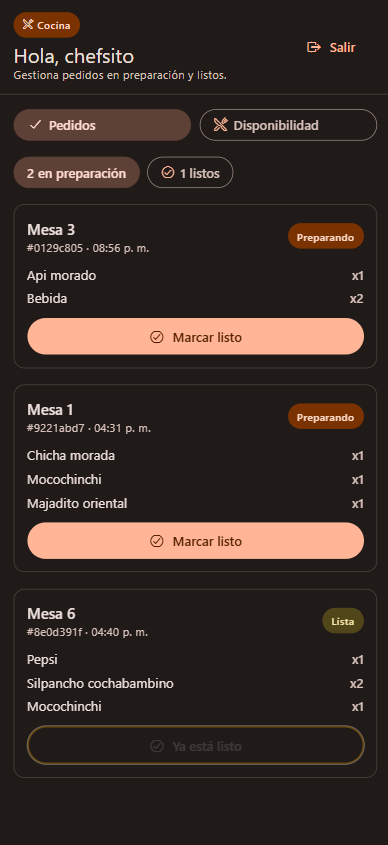
\includegraphics[width=0.92\linewidth]{img/chef-home.png}
  \end{minipage}
  \hfill
  \begin{minipage}{0.48\textwidth}
    \centering
    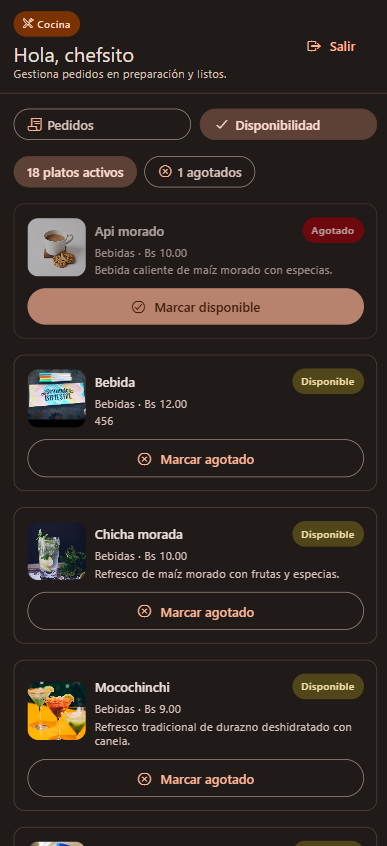
\includegraphics[width=0.92\linewidth]{img/chef-menu.png}
  \end{minipage}
  \caption{Panel de cocina y control de disponibilidad de platos.}
\end{figure}

\subsection{Flujo de Cliente}

Las rutas públicas permiten que el cliente consulte la carta digital o acceda a la
vista de mesa mediante QR. La carta pública validada usa la ruta local
\texttt{/menu/jimmy}; la vista de mesa permite ver el menú y llamar al mesero sin
crear una cuenta.

\begin{figure}[H]
  \centering
  \begin{minipage}{0.48\textwidth}
    \centering
    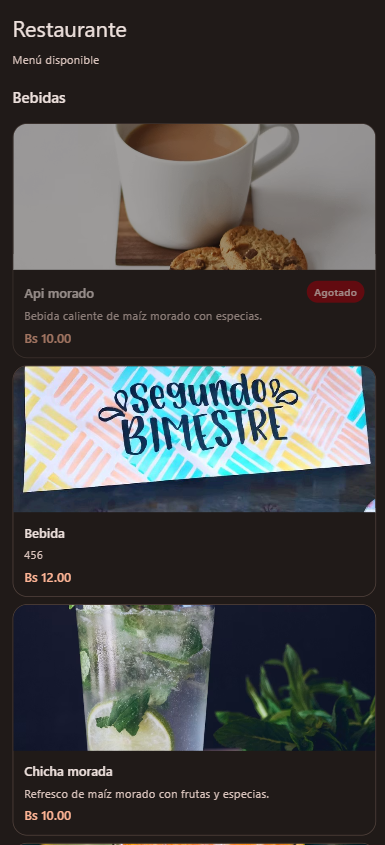
\includegraphics[width=0.92\linewidth]{img/cliente-menu.png}
  \end{minipage}
  \hfill
  \begin{minipage}{0.48\textwidth}
    \centering
    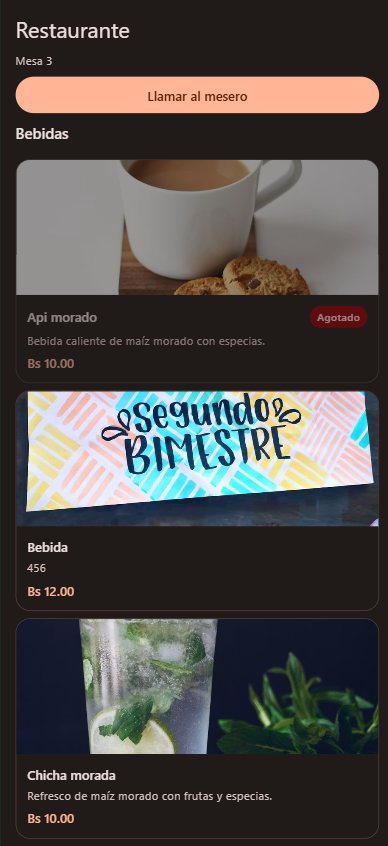
\includegraphics[width=0.92\linewidth]{img/cliente-mesa.png}
  \end{minipage}
  \caption{Carta pública del restaurante y vista pública de mesa con llamada al mesero.}
\end{figure}

\subsection{Control de Versiones}

El repositorio del proyecto se encuentra alojado en GitHub. La captura evidencia la
existencia del repositorio y el QR facilita el acceso directo al código fuente.

\begin{figure}[H]
  \centering
  \begin{minipage}{0.58\textwidth}
    \centering
    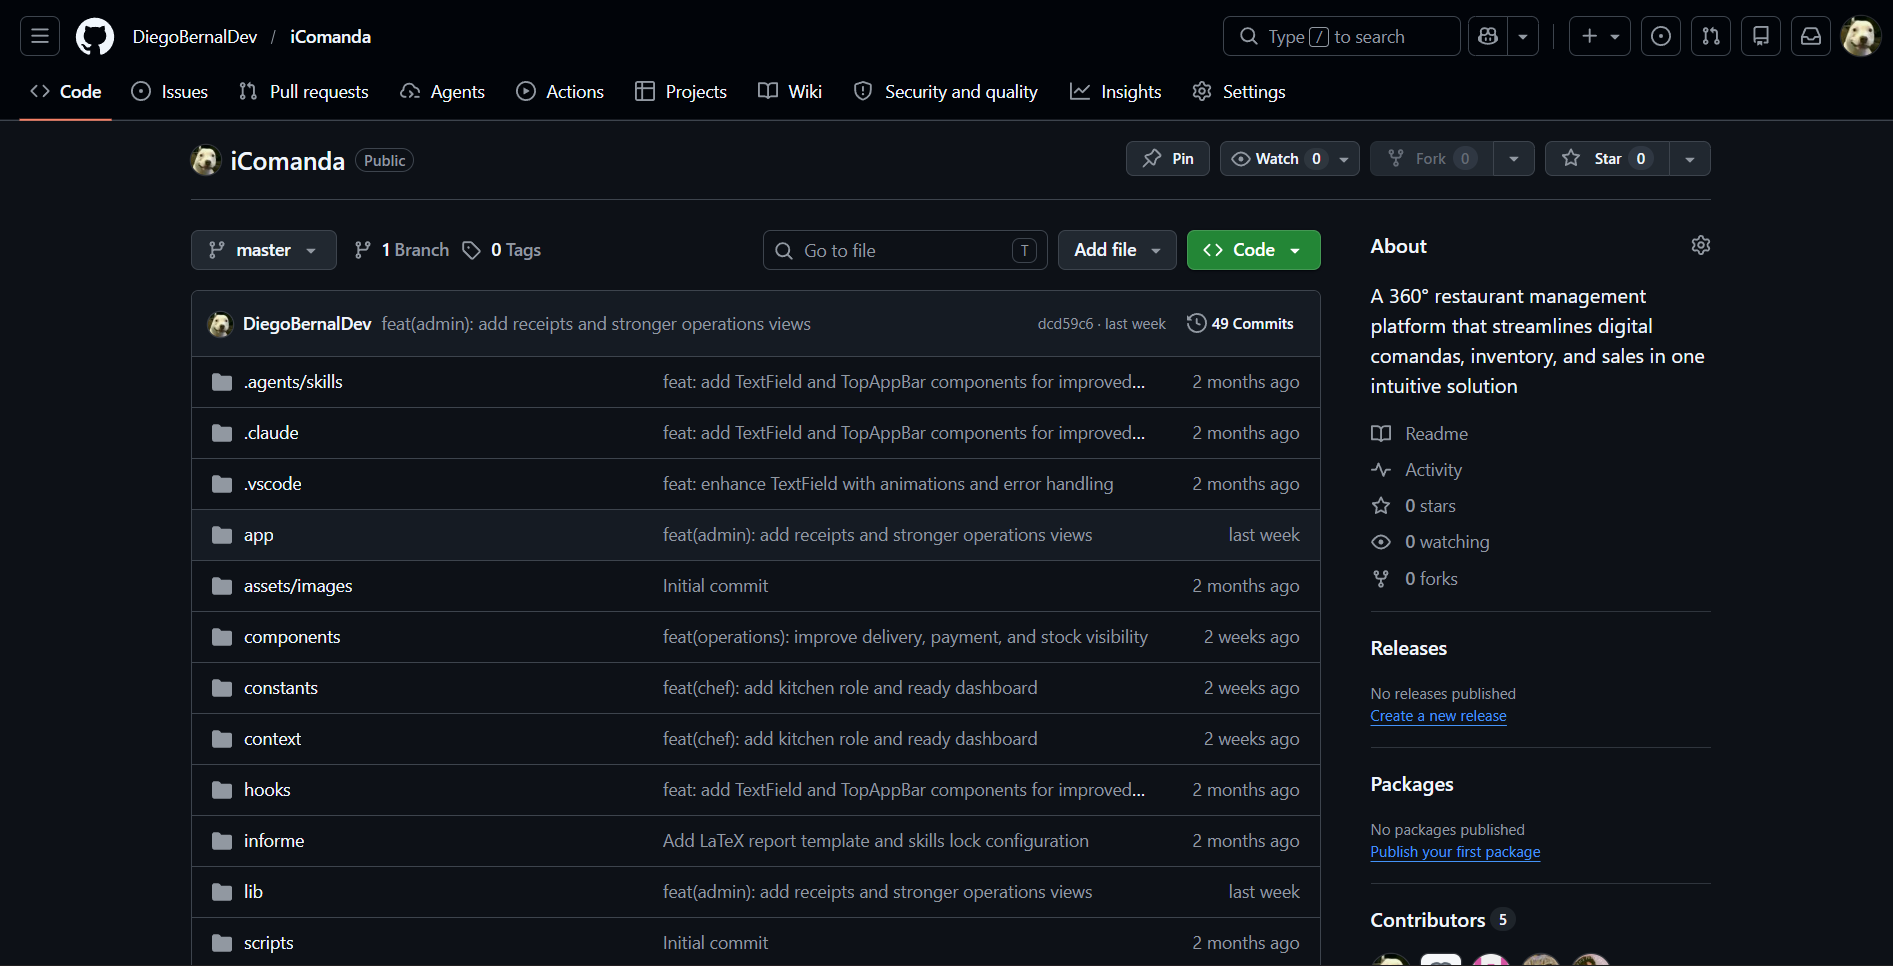
\includegraphics[width=0.95\linewidth]{img/repositorio-captura.png}
  \end{minipage}
  \hfill
  \begin{minipage}{0.34\textwidth}
    \centering
    
\includegraphics[width=0.75\linewidth]{img/qr-repo.png}
  \end{minipage}
  \caption{Repositorio del proyecto en GitHub y QR de acceso: \url{https://github.com/DiegoBernalDev/iComanda.git}.}
\end{figure}

\section{Resultados Obtenidos}

Las pruebas funcionales permitieron validar que los roles principales acceden a sus
módulos correspondientes y que las rutas públicas del cliente funcionan sin inicio
de sesión. También se verificó la integración con Supabase para lectura de menú,
registro de llamadas de mesa, gestión de órdenes, reportes e inventario.

\section{Mejoras Propuestas}

\begin{enumerate}[leftmargin=1.8em]
  \item Integrar una pasarela de pagos para automatizar la confirmación de QR.
  \item Incorporar pruebas automatizadas unitarias y end-to-end.
  \item Añadir modo offline básico para pedidos activos.
  \item Mejorar analítica de inventario con alertas y proyección de consumo.
  \item Agregar monitoreo de errores en producción con una herramienta especializada.
\end{enumerate}
